% This file was created with tikzplotlib v0.9.15.
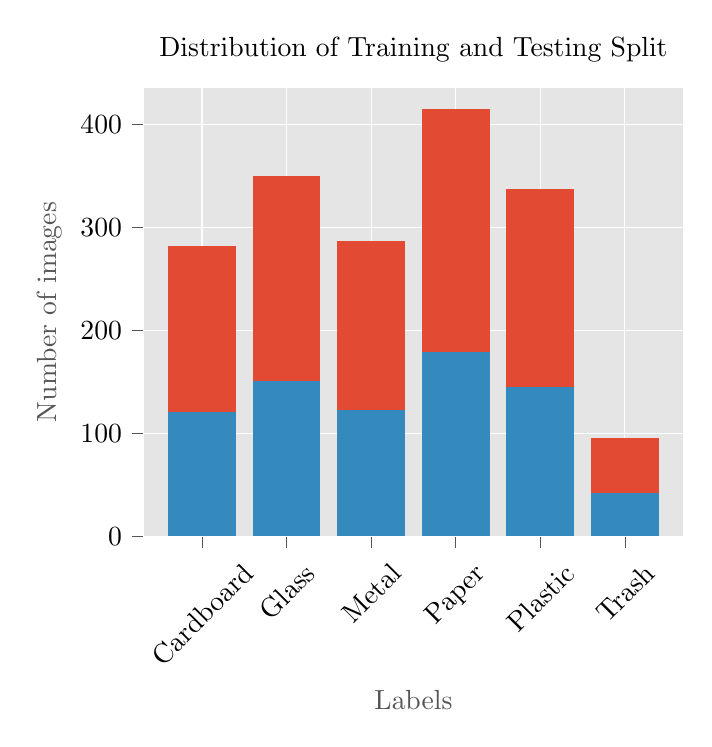
\begin{tikzpicture}

\definecolor{color0}{rgb}{0.886274509803922,0.290196078431373,0.2}
\definecolor{color1}{rgb}{0.203921568627451,0.541176470588235,0.741176470588235}

\begin{axis}[
axis background/.style={fill=white!89.8039215686275!black},
axis line style={white},
legend cell align={left},
legend style={
  fill opacity=0.8,
  draw opacity=1,
  text opacity=1,
  draw=white!80!black,
  fill=white!89.8039215686275!black
},
tick align=outside,
tick pos=left,
title={Distribution of Training and Testing Split},
x grid style={white},
xlabel=\textcolor{white!33.3333333333333!black}{Labels},
xmajorgrids,
xmin=-0.69, xmax=5.69,
xtick style={color=white!33.3333333333333!black},
xtick={0,1,2,3,4,5},
xticklabel style={rotate=45.0},
xticklabels={Cardboard,Glass,Metal,Paper,Plastic,Trash},
y grid style={white},
ylabel=\textcolor{white!33.3333333333333!black}{Number of images},
ymajorgrids,
ymin=0, ymax=435.75,
ytick style={color=white!33.3333333333333!black}
]
\draw[draw=none,fill=color0,very thin] (axis cs:-0.4,0) rectangle (axis cs:0.4,282);
\draw[draw=none,fill=color0,very thin] (axis cs:0.6,0) rectangle (axis cs:1.4,350);
\draw[draw=none,fill=color0,very thin] (axis cs:1.6,0) rectangle (axis cs:2.4,287);
\draw[draw=none,fill=color0,very thin] (axis cs:2.6,0) rectangle (axis cs:3.4,415);
\draw[draw=none,fill=color0,very thin] (axis cs:3.6,0) rectangle (axis cs:4.4,337);
\draw[draw=none,fill=color0,very thin] (axis cs:4.6,0) rectangle (axis cs:5.4,95);
\draw[draw=none,fill=color1,very thin] (axis cs:-0.4,0) rectangle (axis cs:0.4,121);
\draw[draw=none,fill=color1,very thin] (axis cs:0.6,0) rectangle (axis cs:1.4,151);
\draw[draw=none,fill=color1,very thin] (axis cs:1.6,0) rectangle (axis cs:2.4,123);
\draw[draw=none,fill=color1,very thin] (axis cs:2.6,0) rectangle (axis cs:3.4,179);
\draw[draw=none,fill=color1,very thin] (axis cs:3.6,0) rectangle (axis cs:4.4,145);
\draw[draw=none,fill=color1,very thin] (axis cs:4.6,0) rectangle (axis cs:5.4,42);
\end{axis}

\end{tikzpicture}
